\documentclass[11pt,]{article}

\usepackage{amsmath}
\usepackage{amssymb}  % Math

\usepackage[utf8]{inputenc}

\providecommand{\tightlist}{%
	\setlength{\itemsep}{0pt}\setlength{\parskip}{0pt}}

%\setcounter{secnumdepth}{0}

\usepackage{longtable,booktabs}

\usepackage{graphicx,grffile}
\makeatletter
\def\maxwidth{\ifdim\Gin@nat@width>\linewidth\linewidth\else\Gin@nat@width\fi}
\def\maxheight{\ifdim\Gin@nat@height>\textheight\textheight\else\Gin@nat@height\fi}
\makeatother
% Scale images if necessary, so that they will not overflow the page
% margins by default, and it is still possible to overwrite the defaults
% using explicit options in \includegraphics[width, height, ...]{}
\setkeys{Gin}{width=\maxwidth,height=\maxheight,keepaspectratio}



\title{Using the SWIID in Stata  }

\usepackage{fullpage}
\usepackage{setspace}
\usepackage{lscape}
\usepackage{hanging}
\setlength{\tabcolsep}{1pt}

\def\urltilda{\kern -.15em\lower .7ex\hbox{\~{}}\kern .04em}

%\setlength{\textwidth}{6.5in}
%\renewcommand{\footnotesize}{\normalsize}


\renewcommand\floatpagefraction{.9}
\renewcommand\topfraction{.9}
\renewcommand\bottomfraction{.9}
\renewcommand\textfraction{.1}
\setcounter{totalnumber}{50}
\setcounter{topnumber}{50}
\setcounter{bottomnumber}{50}

\def\urltilda{\kern -.15em\lower .7ex\hbox{\~{}}\kern .04em}


\usepackage{natbib}
\bibliographystyle{ajps}



\makeatletter
\@ifpackageloaded{hyperref}{}{%
\ifxetex
  \usepackage[setpagesize=false, % page size defined by xetex
              unicode=false, % unicode breaks when used with xetex
              xetex, colorlinks=true, urlcolor=blue, linkcolor=black, citecolor=black]{hyperref}
\else
  \usepackage[unicode=true, colorlinks=true, urlcolor=blue, linkcolor=black, citecolor=black]{hyperref}
\fi
}
\@ifpackageloaded{color}{
    \PassOptionsToPackage{usenames,dvipsnames}{color}
}{%
    \usepackage[usenames,dvipsnames]{color}
}
\makeatother


\bibpunct{(}{)}{;}{a}{}{,}



\usepackage{amsthm}
\newtheorem{theorem}{Theorem}[section]
\newtheorem{lemma}{Lemma}[section]
\theoremstyle{definition}
\newtheorem{definition}{Definition}[section]
\newtheorem{corollary}{Corollary}[section]
\newtheorem{proposition}{Proposition}[section]
\theoremstyle{definition}
\newtheorem{example}{Example}[section]
\theoremstyle{remark}
\newtheorem*{remark}{Remark}
\begin{document}
	
% \pagenumbering{arabic}% resets `page` counter to 1 
%
% \maketitle

{\title{Using the SWIID in Stata}
	\author{
		Frederick Solt\\
		Associate Professor of Political Science\\
		University of Iowa\\
		\href{mailto:frederick-solt@uiowa.edu}{frederick-solt@uiowa.edu}}
	\date{}
	\maketitle}




\noindent \singlespacing The Standardized World Income Inequality Database (SWIID) uses a custom
missing-data multiple-imputation algorithm to standardize observations
collected from the
\href{http://www.wider.unu.edu/research/Database/}{United Nations
University's World Income Inequality Database version 2.0c}, the
\href{http://www.oecd.org/social/inequality.htm}{OECD Income
Distribution Database}, the
\href{http://sedlac.econo.unlp.edu.ar/eng/}{Socio-Economic Database for
Latin America and the Caribbean generated by CEDLAS and the World Bank},
the \href{http://epp.eurostat.ec.europa.eu}{Eurostat}, the
\href{http://iresearch.worldbank.org/PovcalNet/index.htm}{World Bank's
PovcalNet}, the
\href{http://interwp.cepal.org/sisgen/ConsultaIntegrada.asp?idIndicador=250\&idioma=e}{UN
Economic Commission for Latin America and the Caribbean}, national
statistical offices around the world, and many other sources.
\href{http://www.lisdatacenter.org}{Luxembourg Income Study} data serves
as the standard.

As described in \citet{Solt2016}, the SWIID maximizes the comparability
of available income inequality data for the broadest possible sample of
countries and years. But incomparability remains, and it is sometimes
substantial. This remaining incomparability is reflected in the standard
errors of the SWIID estimates, making it absolutely crucial to take this
uncertainty into account when making comparisons across countries or
over time
\citetext{\citealp[p.238]{Solt2009}; \citealp[p.14]{Solt2016}}. Using
older versions of the SWIID, however, incorporating the standard errors
into an analysis required considerable effort. It is now
straightforward.

Beginning with version 5.0 of the SWIID, the inequality estimates and
their associated uncertainty are represented by 100 separate imputations
of the complete series: for any given observation, the differences
across these imputations capture the uncertainty in the estimate. The
\texttt{SWIIDv5\_1.zip} includes the file \texttt{SWIIDv5\_1.dta}, which
is pre-formatted to facilitate taking this uncertainty into account. The
following sections describe how to subset the data, merge in additional
variables, and do analyses.

\section{Getting Started}\label{getting-started}

The \texttt{SWIIDv5\_1.dta} file is pre-formatted for use with Stata's
tools for analyzing multiply imputed data. Estimates of each of four
inequality measures and their associated uncertainty are represented by
a placeholder variable (which has the measure's name but only missing
data for all observations) plus 100 separate variables (prefixed with
\texttt{\_1\_}, \texttt{\_2\_}, etc.): for any given observation, the
differences across these 100 variables capture the uncertainty in the
estimate.

The four measures are:

\begin{itemize}
\tightlist
\item
  \texttt{gini\_net}: Estimate of Gini index of inequality in
  equivalized (square root scale) household disposable (post-tax,
  post-transfer) income, using
  \href{http://www.lisdatacenter.org}{Luxembourg Income Study} data as
  the standard.
\item
  \texttt{gini\_market}: Estimate of Gini index of inequality in
  equivalized (square root scale) household market (pre-tax,
  pre-transfer) income, using
  \href{http://www.lisdatacenter.org}{Luxembourg Income Study} data as
  the standard.
\item
  \texttt{abs\_red}: Estimated absolute redistribution, the number of
  Gini-index points market-income inequality is reduced due to taxes and
  transfers: the difference between the \texttt{gini\_market} and
  \texttt{gini\_net}.
\item
  \texttt{rel\_red}: Estimated relative redistribution, the percentage
  reduction in market-income inequality due to taxes and transfers: the
  difference between the \texttt{gini\_market} and \texttt{gini\_net},
  divided by \texttt{gini\_market}, multiplied by 100.
\end{itemize}

This format facilitates taking the uncertainty in its estimates into
account when conducting analyses, as will be discussed below. It does
not, however, lend itself easily to tasks such plotting. The
mean-plus-standard-error summary format is much better suited to such
purposes. The following code demonstrates how to put the SWIID in this
summary format, as well as how to make a scatterplot with confidence
intervals.

\begin{verbatim}


. use SWIIDv5_1.dta, clear
(SWIID v5.1, July 2016. Refer to the stata_swiid.pdf file for usage instruction
> s.)

. // Summarize the dataset
. keep country year _*

. 
. foreach v in gini_net gini_market rel_red abs_red {
  2.     egen `v' = rowmean(_*`v')
  3.     egen `v'_se = rowsd(_*`v')
  4.     gen `v'_95ub = `v' + 1.96*`v'_se
  5.     gen `v'_95lb = `v' - 1.96*`v'_se
  6. }
(2064 missing values generated)
(2064 missing values generated)
(2,064 missing values generated)
(2,064 missing values generated)
(2064 missing values generated)
(2064 missing values generated)
(2,064 missing values generated)
(2,064 missing values generated)

. drop _*

. sort country year

. 
. // A silly example
. gen name_length = length(country)

. gen first_letter = substr(country, 1, 1)

. keep if year==2010 & first_letter=="S" /*2010 for Senegal, Serbia, . . .*/
(4,071 observations deleted)

. 
. // A scatterplot with 95% confidence intervals
. twoway rspike gini_net_95ub gini_net_95lb name_length, lstyle(ci) || ///
>     scatter gini_net name_length, msize(small) ///
>     legend(order(2 "SWIID Net-Income Inequality")) 

. 
. graph export stata_scatter.png, replace //export the plot into a png file
(file stata_scatter.png written in PNG format)
\end{verbatim}

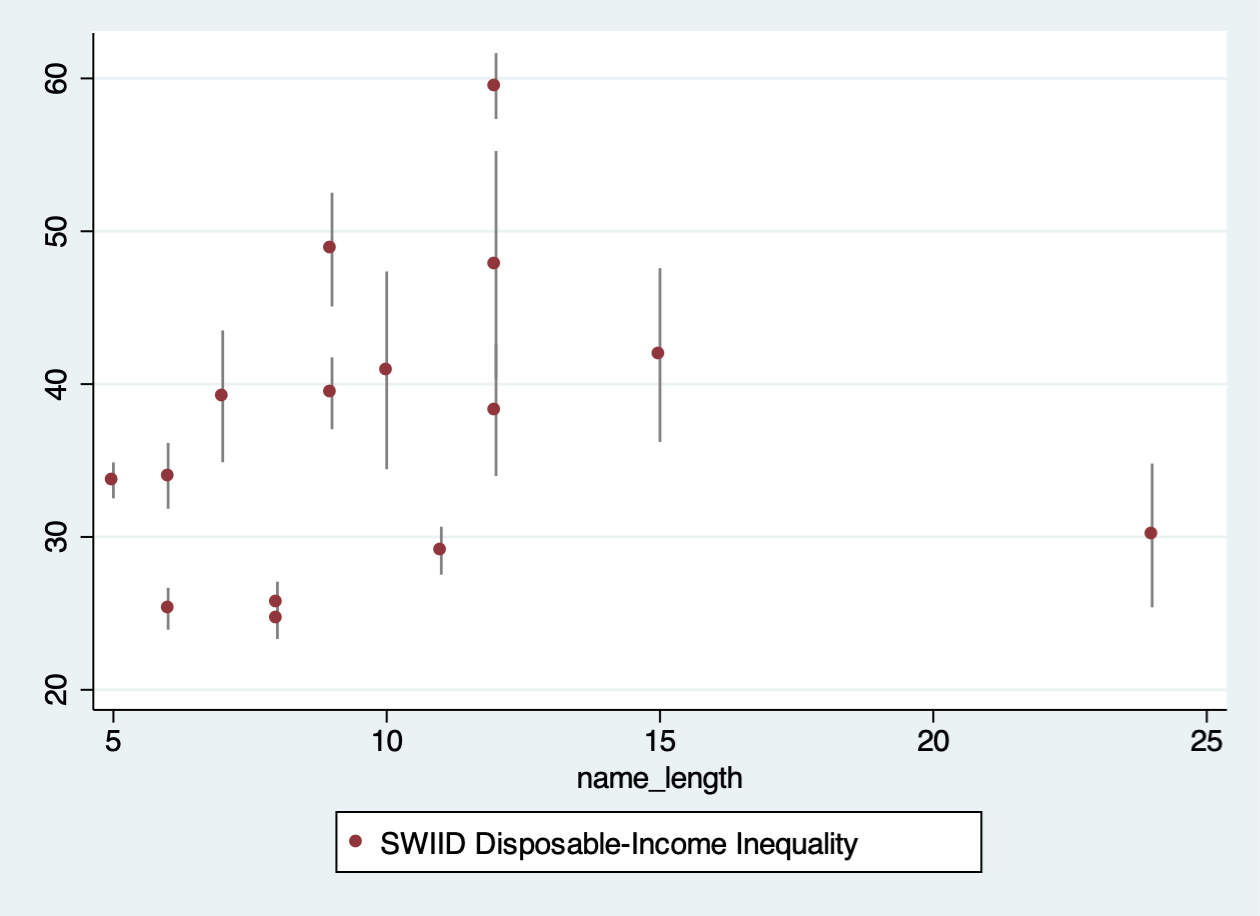
\includegraphics[width=6.54in]{stata_scatter}

\section{Adding Variables}\label{adding-variables}

Generating new variables from the SWIID estimates requires a bit of
care. To preserve Stata's recognition of how the SWIID is formatted for
analysis, the \texttt{mi\ passive:} prefix must be used. Suppose we
wanted to generate a variable for the log of \texttt{gini\_net}. For
this new variable to take into account the uncertainty in the SWIID
estimates, instead of simply typing
\texttt{gen\ ln\_gini\_net\ =\ ln(gini\_net)}, we need to preface that
command with the \texttt{mi\ passive:} prefix, as below:

\begin{verbatim}
mi passive: gen ln_gini_net = ln(gini_net)
\end{verbatim}

The result is a placeholder variable for the new measure
\texttt{ln(gini\_net)}, plus 100 separate variables prefixed with
\texttt{\_1\_}, \texttt{\_2\_}, etc. that together represent the
uncertainty in our new measure. Note that there is no need to use
\texttt{mi\ passive:} to create variables in the dataset that are not
based on the SWIID estimates.

\section{Merging}\label{merging}

To merge the SWIID and additional data, simply merge the other dataset
\emph{into} the SWIID dataset. Note that this means that the SWIID
should be the `master' file in the merge, the other data should be the
`using' file.

Suppose we wanted to do a (simplified) replication of Solt, Habel, and
Grant's analysis \citeyearpar{Solt2011} of
\href{http://worldvaluessurvey.org}{World Values Survey} data on
religiosity. As our measure of religiosity, we will use the WVS item on
respondents' self-report of the importance of God to their lives, which
is measured on a ten-point scale. Given secularization theory, we will
need to control for GDP per capita, which we will calculate from
information from the \href{http://www.ggdc.net/pwt}{Penn World Tables}
\citep{Feenstra2015}. Below we first load the PWT dataset and use it to
generate a dataset of GDP per capita (in thousands of dollars). Then we
load the WVS data, generate our variables of interest, and merge in our
PWT data. Finally, we merge these data into the SWIID.

\begin{verbatim}
// Get GDP per capita data from the Penn World Tables, Version 9.0 (Feenstra et al. 2015)
// download from http://www.rug.nl/research/ggdc/data/pwt/v90/pwt90.xlsx
// create gdppc and save as .dta

import excel using pwt90.xlsx, sheet("Data") firstrow clear
gen gdppc = rgdpe/pop/1000
drop if gdppc==.
keep country year gdppc
save pwt90_gdppc.dta, replace

// Get World Values Survey 6-wave data 
// from http://www.worldvaluessurvey.org/WVSDocumentationWVL.jsp
// generate variables of interest, merge in the PWT data, and save
use WVS_Longitudinal_1981_2014_stata_v2015_04_18.dta, clear
kountry S003, from(iso3n)
rename NAMES_STD country
gen year = S020
gen religiosity = F063 if F063>0
gen age = X003 if X003>0
gen educ = X025 if X025>0
gen male = (X001 == 1) if X001>0
keep country year religiosity male educ age

merge m:1 country year using pwt90_gdppc.dta
drop if _merge!=3
drop _merge
save wvs_pwt.dta, replace

// Now merge these data *into* the SWIID
use SWIIDv5_1.dta, clear
merge 1:m country year using wvs_pwt.dta
drop if _merge!=3
drop _merge
\end{verbatim}

\section{Analyzing}\label{analyzing}

Once any additional variables are created or merged in, we may proceed
to analysis. Continuing with our example, we estimate a three-level
linear mixed-effects model of individual responses nested in
country-years nested in countries using \texttt{mixed}. To take the
uncertainty in the SWIID estimates into account, we construct our model
comman as usual, but precede it with the \texttt{mi\ estimate:} prefix
to perform it on each of the 100 variables that report the uncertainty
in the SWIID estimates. Note that performing an analysis 100 times can
be time-consuming.

\begin{verbatim}
mi estimate: mixed religiosity gini_net gdppc age educ male || country: || country_year:
\end{verbatim}

\section{Citing the SWIID}\label{citing-the-swiid}

Please cite to the SWIID by referring to its article of record and
including the version number and date of release:

\begin{quote}
Solt, Frederick. 2016. ``The Standardized World Income Inequality
Database.'' \emph{Social Science Quarterly} 97. SWIID Version 5.1, July
2016.
\end{quote}

\newpage
\singlespacing 
\bibliography{swiid}




\end{document}
